\chapter{Desenvolvimento do Projeto}

O projeto do sistema de iluminação controlado pela internet foi desenvolvido com o objetivo de apresentar algumas funcionalidades e demonstrar a potencialidade de economia de energia. As funcionalidades propostas foram as de, remotamente, ligar e desligar a iluminação; apresentar dois modos de controle da luminosidade: O modo normal no qual o usuário poderá escolher a intensidade da fita de LED e o modo econômico no qual o sistema levará em conta a iluminação ambiente para manter um nível mínimo, definido pelo usuário, de luminosidade. A demonstração da economia de energia do sistema é baseada na comparação das estimativas do consumo da iluminação com intensidade máxima e do consumo com intensidade controlada automaticamente.

\section{Montagem}

Os principais componentes e materiais usados no projeto já foram descritos no capítulo 3. O esquema elétrico foi pensado com o objetivo de fazer com que o sistema atendesse às funcionalidades propostas.

% FIGURA NO FRITZING DA PROTOBOARD

A lista completa de materiais usados no projeto:

\begin{table}
    \centering
    \caption{Lista de materiais}
    \label{BOM}
    \begin{tabular}{ll} 
        \hline
        Material                                                       & Quantidade  \\ 
        \hline
        \hline
        Fonte de chaveada 220VAC \textasciitilde{} 12VDC/2A            & 1           \\ 
        \hline
        Kit de regulador para \textit{protoboard} baseado no CI LM1117 & 1           \\ 
        \hline
        \textit{Wemos~}D1 Mini                                         & 1           \\ 
        \hline
        Fita de LED branca 3528 12V 4.8W/m                             & 1           \\ 
        \hline
        Sensor de Luminosidade LDR 5mm                                 & 1           \\ 
        \hline
        TIP122 Transistor \textit{Darlington} NPN                      & 1           \\ 
        \hline
        Resistor $10K\Omega$                                           & 1           \\ 
        \hline
        Resistor $220\Omega$                                           & 1           \\ 
        \hline
        Conector P4 macho                                              & 1           \\
        \hline
    \end{tabular}
\end{table}

O esquema eletrônico dos componentes é mostrado na Figura X e ilustrado na Figura Y conforme montado na \textit{protoboard}.

FIGURA X ESQUEMATICO

FIGURA Y PROTOBOARD

\section{Programação}

\lstset{
    frame=tb,
    language=C++,
    aboveskip=3mm,
    belowskip=3mm,
    showstringspaces=false,
    columns=flexible,
    basicstyle={\small\ttfamily},
    numbers=left,                    
    numbersep=5pt,                  
    numberstyle=\tiny\color{gray},
    keywordstyle=\color{blue},
    commentstyle=\color{dkgreen},
    stringstyle=\color{mauve},
    breaklines=true,
    breakatwhitespace=true,
    tabsize=4,
    captionpos=b
}

Conforme descrito no capítulo 3, a codificação do microcontrolador foi desenvolvida usando a linguagem "C++" compilado com a extensão do \textit{Arduino} junto com as bibliotecas e compilador oficiais da \textit{Espressif}. O código foi escrito no ambiente \textit{Visual Studio Code} com a ferramenta de sistemas embarcados \textit{PLatformIO}.

\subsection{Cabeçalho}

O cabeçalho do código contém declarações de bibliotecas, variáveis, constantes e macros.

\begin{lstlisting}

/************************** Libraries ***************************/
#include <Arduino.h>
#include <ESP8266WiFi.h>
#include "Adafruit_MQTT.h"
#include "Adafruit_MQTT_Client.h"

// Includes do Wifi Manager
#include <DNSServer.h>
#include <ESP8266WebServer.h>
#include <WiFiManager.h>         //https://github.com/tzapu/WiFiManager

/********************* WiFi Access Point *************************/

#define WLAN_SSID       "GVT-4238"
#define WLAN_PASS       "6703003118"

/********************* Adafruit.io Setup *************************/

#define AIO_SERVER      "io.adafruit.com"
#define AIO_SERVERPORT  1883
#define AIO_USERNAME    "RafaelMQ"
#define AIO_KEY         "f6ed222e222c446088110578b7bd0146"

/********************* PIN DEFINITIONS **************************/
#define USER_LED D1

#define pwm_map_n(x) round(map(x, 0, 100, 0, 1023))

/************** GLOBAL STATE (don't change this!) ***************/

// Create an ESP8266 WiFiClient class to connect to the MQTT server.
WiFiClient client;

// Setup the MQTT client class by passing in the WiFi client and MQTT server and login details.
Adafruit_MQTT_Client mqtt(&client, AIO_SERVER, AIO_SERVERPORT, AIO_USERNAME, AIO_USERNAME, AIO_KEY);

/************************ Feeds ********************************/

Adafruit_MQTT_Subscribe timefeed = Adafruit_MQTT_Subscribe(&mqtt, "time/seconds");

// Setup a feed called 'pwmin' for subscribing to changes on the slider
Adafruit_MQTT_Subscribe pwmin = Adafruit_MQTT_Subscribe(&mqtt, AIO_USERNAME "/feeds/pwmin");

// Setup a feed called 'onoff' for subscribing to changes to the button
Adafruit_MQTT_Subscribe onoffbutton = Adafruit_MQTT_Subscribe(&mqtt, AIO_USERNAME "/feeds/onoff");

Adafruit_MQTT_Publish pwmout = Adafruit_MQTT_Publish(&mqtt, AIO_USERNAME "/feeds/pwmout");

/********************* Variables *****************************/
int sec;
int minute;
int hour;

int timeZone = -3; // utc-3 eastern daylight time (brasilia)

int global_pwm = 100;
bool led_state = false;

\end{lstlisting}

As definições da seção \textit{"Adafruit.io Setup"} são dados próprios da conta do usuário do serviço da \textit{Adafruit}. As declarações da seção \textit{"Global State"} configuram o sistema na rede MQTT do serviço da \textit{Adafruit}. A seção de \textit{"Feeds"} se baseia nos exemplos da documentação de MQTT da \textit{Adafruit} e declara objetos das classes \textit{Subscribe} e \textit{Publish}. E na seção \textit{"Variables"} temos a declaração das variáveis usadas no código.

\subsection{Função \textit{setup()}}

A função \textit{setup()} é chamada no começo da execução do programa apenas uma vez, por isso é responsável por realizar configurações e preparações para o restante da execução do programa.

\begin{lstlisting}
void setup() {
    pinMode(USER_LED, OUTPUT);
    Serial.begin(115200);
    delay(10);

    Serial.println("Lampada mqtt");

    // Connect to WiFi access point. 
    // WiFiManager.
    // Local intialization. Once its business is done, there is no need to keep it around
    Serial.println();
    Serial.print("Connecting ");

    WiFiManager wifiManager;
    wifiManager.autoConnect("Fita de LED MQTT", "2018");

    Serial.println("WiFi connected");
    Serial.println("IP address: "); 
    Serial.println(WiFi.localIP());
    Serial.printf(" ESP8266 Chip id = \%08X\n", ESP.getChipId());
    
    // Setup subscribes callbacks
    timefeed.setCallback(timecallback);
    pwmin.setCallback(pwmincallback);
    onoffbutton.setCallback(onoffcallback);

    // Setup MQTT subscriptions.
    mqtt.subscribe(&timefeed);
    mqtt.subscribe(&pwmin);
    mqtt.subscribe(&onoffbutton);
}
\end{lstlisting}

Inicialmente são inicializados a comunicação serial, que não interfere no funcionamento do sistema e é usada apenas para depuração, e os pinos de entrada e saída, com exceção do pino de entrada analógica pois este têm esta função por padrão e sua inicialização pode ser dispensada se for usada para este propósito. Posteriormente, é executada a rotina de conexão com o uso da função da biblioteca \textit{"WiFiManager"} \cite{wifimng} que tenta se conectar a última rede a qual havia se conectado anteriormente, ao checar o campo da memória reservada para guardar informações de \textit{"SSID"} e senha; caso não consiga, a função coloca o ESP-8266 na configuração de "ponto de acesso" WiFi, com o \textit{SSID} e senha definidos pelos argumentos da função "wifiManager.autoConnect", e cria uma página \textit{web}, aberta automaticamente ao se conectar ao "ponto de acesso", que permite informar ao sistema qual a rede deve se conectar e a senha dessa rede. E em seguida as funções de \textit{"callbacks"}, que são chamadas quando ocorre uma publicação nos tópicos subscritos, são atreladas aos objetos de subscrição da classe MQTT. Por fim, faz-se a subscrição nos tópicos

\section{Interfaces de Usuário}

O projeto do sistema de iluminação controlado via internet tem duas interfaces de usuário. A interface principal é um aplicativo móvel para o sistema \textit{Android} e a interface \textit{web} é uma funcionalidade oferecida pelo serviço da \textit{Adafruit}.

\subsection{Aplicativo Móvel}

A interface por aplicação móvel para sistemas \textit{Android} usada é baseada no aplicativo "MQTT \textit{Dash}", disponível, gratuitamente, na loja oficial da \textit{Google} \cite{dash}. O aplicativo permite várias interfaces independentes; ao criar uma interface, o usuário define várias características como nome da interface, endereço do servidor MQTT, o número da porta, nome de usuário, senha, e número de linhas e colunas do \textit{layout} da interface. Pode ser criado um atalho na tela inicial do aparelho da interface. Criada a interface o usuário pode criar elementos, denominados \textit{"widgets"}, que podem ser botões, mostradores, e algumas estruturas que permitem escolher um número arbitrário em um intervalo, ou uma estrutura que permita a escolha de uma dentre múltiplas opções predefinidas. Os \textit{widgets} interagem na rede MQTT ao publicar mensagens escolhidas pelo usuário ou predefinidas no aplicativo, mostrar valores recebidos devido a subscrições, ou ainda apresentar determinados comportamentos dependendo da mensagem recebida ou publicada.

A interface criada para este projeto conta com três \textit{widgets}: Um botão para ligar e desligar a iluminação, uma estrutura para escolher um valor de 0 a 100 correspondente a porcentagem da intensidade da iluminação e uma estrutura que permite alternar entre os modos de funcionamento econômico ou normal. Os \textit{widgets} estão sincronizados com a interface \textit{web} por meio da subscrição nos mesmos tópicos em que publicam, isto significa que seu estado muda automaticamente caso haja publicação nesse mesmo tópico.

\begin{figure}[ht]
    \begin{center}
    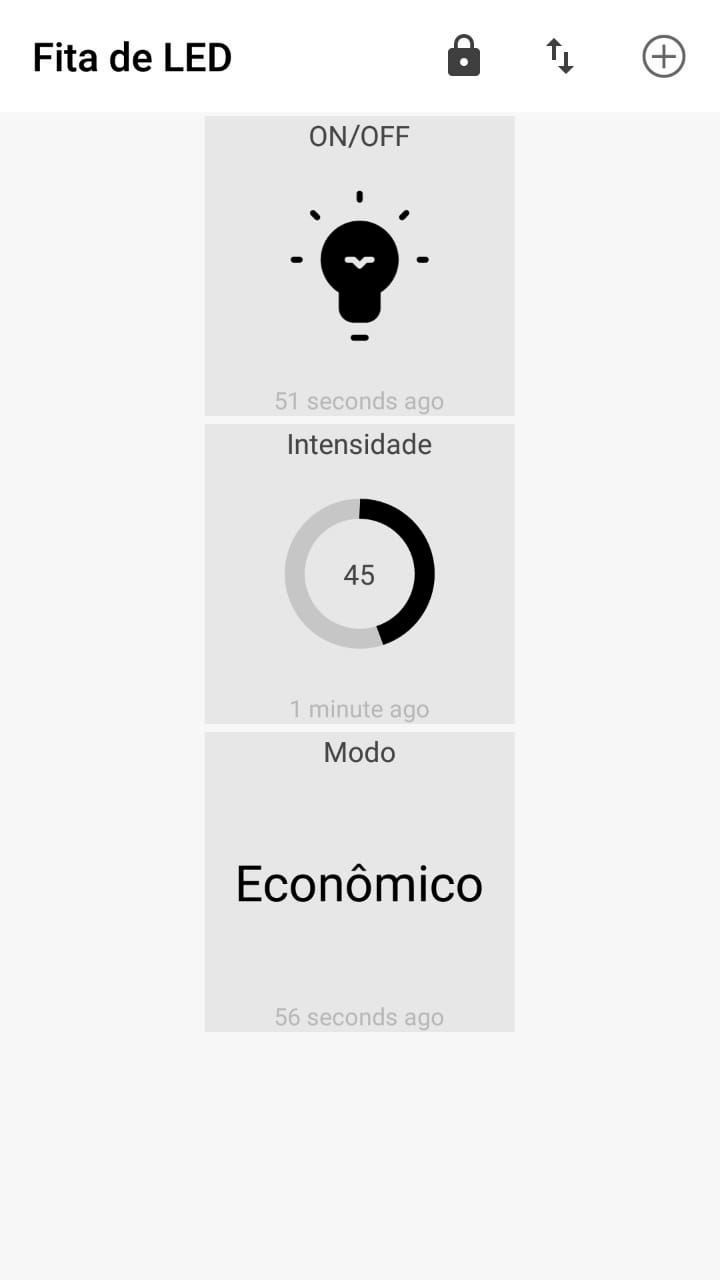
\includegraphics[width=0.4\textwidth]{figuras/appdash.png}
    \end{center}
    \caption[Ilustração do aplicativo móvel.]{Ilustração do aplicativo móvel com cores invertidas para evitar o fundo escuro da imagem.}
    \label{appdash}
\end{figure}

O botão "ON/OFF" pode ligar e desligar a iluminação ao publicar os valores "0" e "1", respectivamente, no tópico \texttt{"RafaelMQ/feeds/onoff"} e apresenta um visual lúdico; quando se encontra no estado "1" mostra a figura de uma "lâmpada acesa" e quando no estado "0" mostra a figura de uma "lâmpada apagada". 

A estrutura que permite arbitrar a intensidade da iluminação, chamado no aplicativo de "\textit{slider}", publica e subscreve no tópico \texttt{"RafaelMQ/feeds/pwmin"} valores inteiros no intervalo de "0" a "100" representando a porcentagem da intensidade máxima. O \textit{widget} "Modo" publica no tópico \texttt{"RafaelMQ/feeds/modo"} e serve para selecionar o modo de funcionamento dentre as opções "Econômico", e "Normal". 

\subsection{Interface \textit{Web}}

A interface \textit{web} é uma das funcionalidades ofertadas pelo serviço da \textit{Adafruit} e têm \textit{widgets} bem parecidos com os do aplicativo móvel; com uma diferença principal: Há um widget que plota um gráfico temporal dos valores publicados em algum dos tópicos e permite que os dados de qualquer tópico possam ser salvos em um arquivo "csv", formato compatível com os principais editores de planilhas.

\begin{figure}[ht]
    \begin{center}
    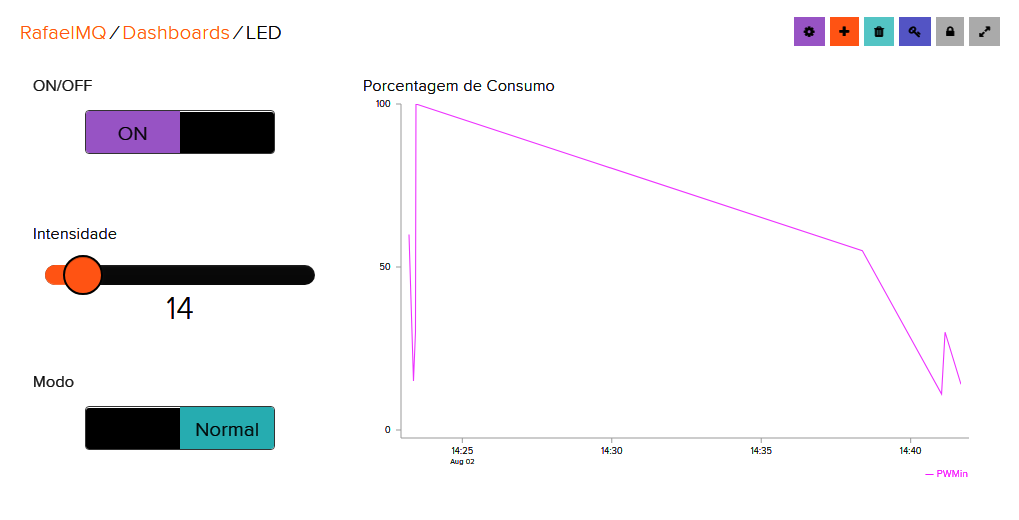
\includegraphics[width=\textwidth]{figuras/adaio.PNG}
    \end{center}
    \caption[Ilustração da interface \textit{web}.]{Ilustração da interface \textit{web} com cores invertidas para evitar o fundo escuro da imagem.}
    \label{adaio}
\end{figure}

O comportamento e funcionamento dos \textit{widgets} da interface \textit{web} é bastante similar ao dos \textit{widgets} da aplicação móvel com as mesmas estruturas de ligar e desligar, alterar a intensidade da iluminação e selecionar o modo de operação.
